\documentclass{article}
\usepackage{graphicx}
\usepackage{amsmath}
\usepackage{hyperref}

\begin{document}

    \title{Questioning the Questions}
    \author{Kilian Lehn}
    \date{\today}
    \maketitle

    \section*{GitHub Repository}
    Repository: \href{https://github.com/kilian-lm/questioning_the_question}{https://github.com/kilian-lm/questioning\_the\_question}
    \label{sec:repository}

    \tableofcontents
    \clearpage


    \section{Introduction}

    This paper presents a model to investigate the dynamics of human questioning behavior and the development of understanding over a lifetime.


    \section{Questioning and Understanding: A Model}
    \label{sec:model}
    Symptom to treat: Our theories often determine our observations, and we tend to observe what confirms our theories, thereby reinforcing our beliefs.
    Antidote: By identifying the boundaries of our mindset, we can challenge and transcend them.
    A two-layered approach is suggested for this purpose:
    \begin{enumerate}
        \item We can understand the dynamics and mechanisms of the human mind's data processing to a certain extent when we compare it in two layers. The second layer is predicated on achieving the first layer, as it requires a broad understanding of personal questioning patterns:
        \begin{itemize}
            \item \textit{First Layer - Local to Global Perception of Own Questioning Patterns}: Questioning is a constant process, and to a certain degree, reality aligns with it. Consequently, our personal reality is substantially shaped by the way we ask questions. This leads to the understanding that questioning is the independent variable, and reality the dependent one. Thus, on the level of the first layer, our prognoses are progressively fine-tuned, not to reality, but to the underlying patterns of how we question reality.
            \item \textit{Second Layer - Establishing Feedback Loops of Global Perception of Own Questioning Patterns to Reality}: Once a comprehensive understanding of personal questioning patterns has been achieved, we can then benchmark these against reality.
        \end{itemize}
    \end{enumerate}
    \label{sec:assumptions}


    \section{Implementation and Further Discussion}

    We propose a Python class \texttt{Person}, which allows us to plot the formulated assumptions up to the second layer.


    \section{Mathematical Model}

    The frequency $F_t$ of questioning at time $t$ is modeled as an exponential decay process with an initial frequency $F_0$ and a rate of change $r_F$:

    \[
        F_t = F_0 \exp(-r_F t)
    \]

    With the understanding that an exponential increase in question quality and an exponential decrease in question frequency lead to a nonlinear progression of understanding, we model the level of understanding $U_t$ at time $t$ with an initial understanding $U_0$ and a rate of increase $r_U$ that is proportional to the product of the quality and frequency of questions:

    \[
        U_t = U_0 + r_U Q_t F_t
    \]

    Where $Q_t$ represents the quality of questions over time, which increases exponentially.

    \begin{figure}[ht]
        \centering
        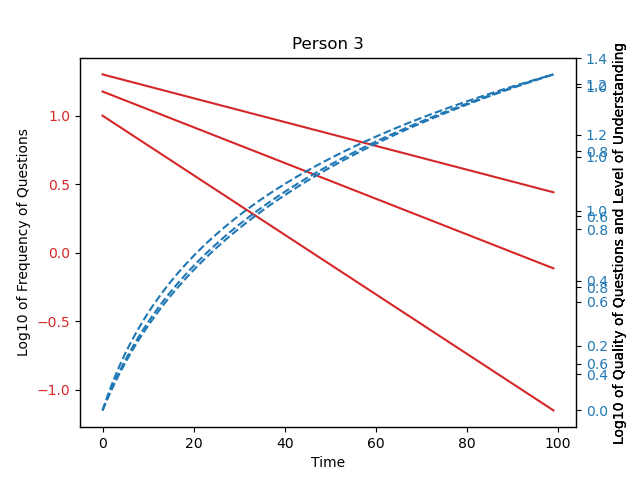
\includegraphics[width=0.7\textwidth]{combined_plot.png}
        \caption{Combined Plot of Persons}
        \label{fig:combinedplot}
    \end{figure}


    \section{Discussion}

    The model provides a highly simplified representation of the complex processes of human questioning and understanding development. Although it does not capture all the nuances of these processes, it offers a starting point for understanding their dynamics and how they might change under different conditions.

    \subsection{Person 1}

    Person 1, who experiences the strongest increase in the quality of questions and level of understanding, sees the largest decrease in the frequency of questions over time. This is based on the correlation that an increase in the quality of questions and level of understanding causes a decrease in the frequency of questions. A similar pattern can be observed for Person 2 and Person 3, though the changes are less pronounced.

    \subsection{Person 2}

    Person 2 exhibits a moderate increase in the quality of questions and level of understanding, resulting in a gradual decrease in the frequency of questions over time. The changes in frequency, quality, and understanding are less pronounced compared to Person 1.

    \subsection{Person 3}

    Person 3 shows a relatively slower increase in the quality of questions and level of understanding. As a result, the decrease in the frequency of questions over time is less significant compared to Person 1 and Person 2.

    \subsection{Perception, Time, and the Pursuit of Eternity}

    In the pursuit of understanding, there comes a time when the questions used in daily life can be located in the global trends of the questioning patterns. This is the point where the second layer mentioned in Section~\ref{sec:assumptions} comes into play. Only when the global trends of our questioning patterns are observable, then we can start to benchmark them against reality. The second layer will be the object of consideration in another paper.

    Here, just to convey the concept of a global trend map of the questioning patterns (see code~\ref{sec:repository}), we present a 3D plot (Figure~\ref{fig:3dplot}):

    \begin{figure}[ht]
        \centering
        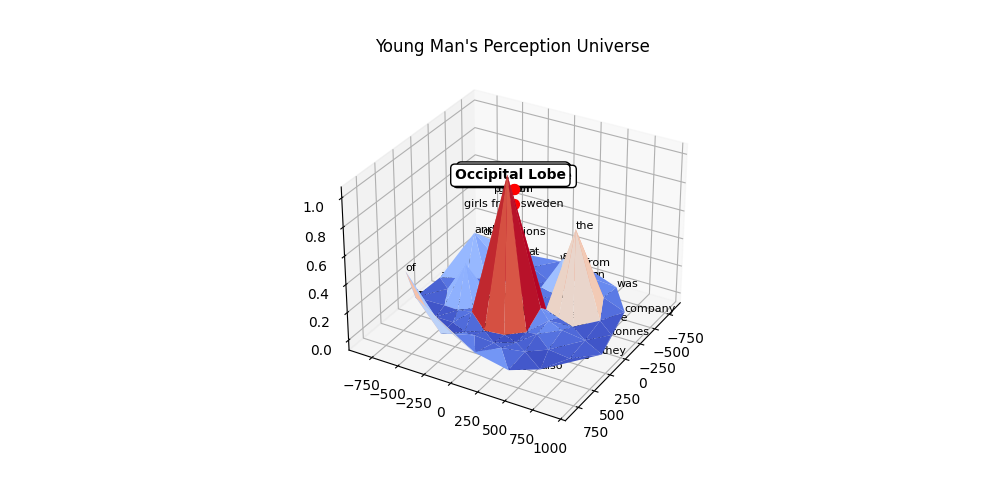
\includegraphics[width=0.7\textwidth]{3d_plot.png}
        \caption{3D Plot}
        \label{fig:3dplot}
    \end{figure}


    \section{Conclusion}

    In a life where an individual fails to recognize patterns and dynamics (single-case-life), the individual is kept in an error-loop, recreating its beliefs. Conversely, in a life where past questioning patterns are recognized, the individual can identify error patterns and challenge those boundaries.
\end{document}




